\documentclass[tikz,border=12pt]{standalone}
\usepackage[T1]{fontenc}
\usepackage{mathpazo}
\usepackage{amsmath,amssymb}
\usetikzlibrary{arrows.meta, positioning, calc, fit, decorations.pathreplacing}

\definecolor{stblue}{HTML}{7B97AD}
\definecolor{rwgold}{HTML}{B8995E}
\definecolor{sage}{HTML}{7A9A7E}
\definecolor{dkbrown}{HTML}{3D3530}
\definecolor{wmgray}{HTML}{7B7067}
\definecolor{cream}{HTML}{F9F6F0}
\definecolor{border}{HTML}{D4C9B8}
\definecolor{terracotta}{HTML}{C47A6A}
\definecolor{lavender}{HTML}{907EA0}

\begin{document}
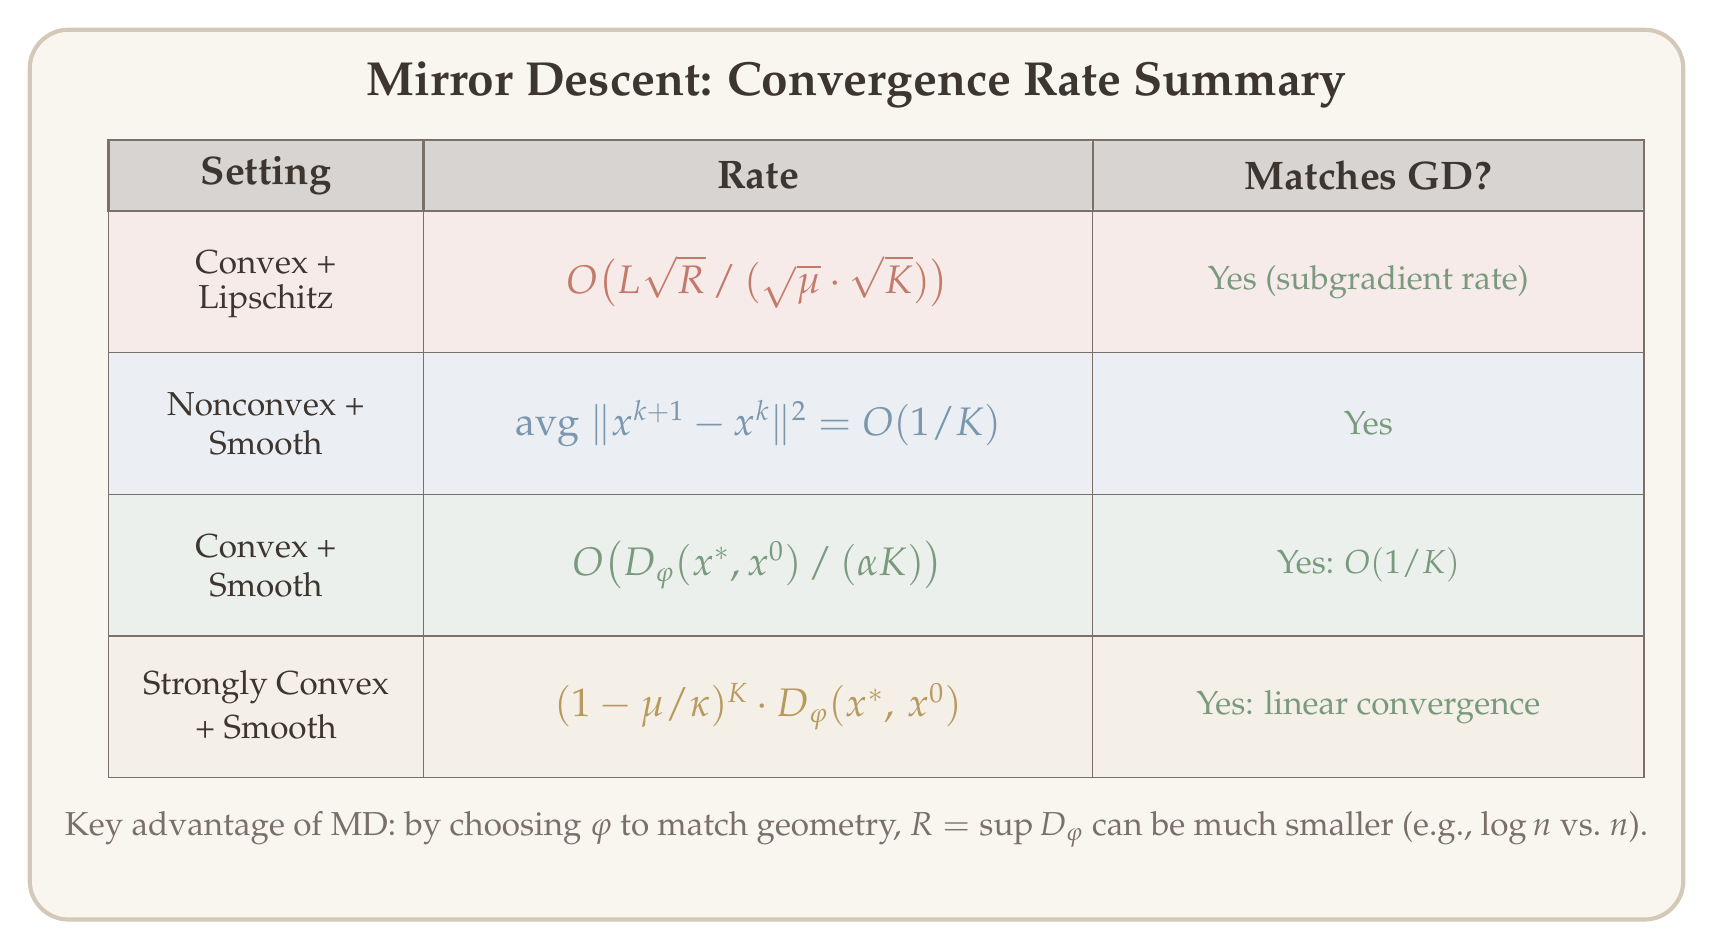
\begin{tikzpicture}[>={Stealth[length=4mm, width=3mm]}]

% Background
\fill[cream, rounded corners=14pt] (-0.5,-0.5) rectangle (20.5,10.8);
\draw[border, line width=1.5pt, rounded corners=14pt] (-0.5,-0.5) rectangle (20.5,10.8);

% Title
\node[text=dkbrown, font=\LARGE\bfseries] at (10,10.1) {Mirror Descent: Convergence Rate Summary};

% Table header
\fill[wmgray!30, rounded corners=2pt] (0.5,8.5) rectangle (4.5,9.4);
\draw[wmgray, line width=0.8pt] (0.5,8.5) rectangle (4.5,9.4);
\node[text=dkbrown, font=\Large\bfseries] at (2.5,8.95) {Setting};

\fill[wmgray!30, rounded corners=2pt] (4.5,8.5) rectangle (13.0,9.4);
\draw[wmgray, line width=0.8pt] (4.5,8.5) rectangle (13.0,9.4);
\node[text=dkbrown, font=\Large\bfseries] at (8.75,8.95) {Rate};

\fill[wmgray!30, rounded corners=2pt] (13.0,8.5) rectangle (20.0,9.4);
\draw[wmgray, line width=0.8pt] (13.0,8.5) rectangle (20.0,9.4);
\node[text=dkbrown, font=\Large\bfseries] at (16.5,8.95) {Matches GD?};

% Row 1: Lipschitz
\fill[terracotta!15] (0.5,6.7) rectangle (4.5,8.5);
\draw[wmgray, line width=0.5pt] (0.5,6.7) rectangle (4.5,8.5);
\node[text=dkbrown, font=\large] at (2.5,7.85) {Convex +};
\node[text=dkbrown, font=\large] at (2.5,7.35) {Lipschitz};

\fill[terracotta!15] (4.5,6.7) rectangle (13.0,8.5);
\draw[wmgray, line width=0.5pt] (4.5,6.7) rectangle (13.0,8.5);
\node[text=terracotta, font=\Large] at (8.75,7.6) {$O\bigl(L\sqrt{R}\,/\,(\sqrt{\mu}\cdot\sqrt{K})\bigr)$};

\fill[terracotta!15] (13.0,6.7) rectangle (20.0,8.5);
\draw[wmgray, line width=0.5pt] (13.0,6.7) rectangle (20.0,8.5);
\node[text=sage, font=\large] at (16.5,7.6) {Yes (subgradient rate)};

% Row 2: Nonconvex + Smooth
\fill[stblue!15] (0.5,4.9) rectangle (4.5,6.7);
\draw[wmgray, line width=0.5pt] (0.5,4.9) rectangle (4.5,6.7);
\node[text=dkbrown, font=\large] at (2.5,6.05) {Nonconvex +};
\node[text=dkbrown, font=\large] at (2.5,5.55) {Smooth};

\fill[stblue!15] (4.5,4.9) rectangle (13.0,6.7);
\draw[wmgray, line width=0.5pt] (4.5,4.9) rectangle (13.0,6.7);
\node[text=stblue, font=\Large] at (8.75,5.8) {avg $\|x^{k+1} - x^k\|^2 = O(1/K)$};

\fill[stblue!15] (13.0,4.9) rectangle (20.0,6.7);
\draw[wmgray, line width=0.5pt] (13.0,4.9) rectangle (20.0,6.7);
\node[text=sage, font=\large] at (16.5,5.8) {Yes};

% Row 3: Convex + Smooth
\fill[sage!15] (0.5,3.1) rectangle (4.5,4.9);
\draw[wmgray, line width=0.5pt] (0.5,3.1) rectangle (4.5,4.9);
\node[text=dkbrown, font=\large] at (2.5,4.25) {Convex +};
\node[text=dkbrown, font=\large] at (2.5,3.75) {Smooth};

\fill[sage!15] (4.5,3.1) rectangle (13.0,4.9);
\draw[wmgray, line width=0.5pt] (4.5,3.1) rectangle (13.0,4.9);
\node[text=sage, font=\Large] at (8.75,4.0) {$O\bigl(D_\varphi(x^*,x^0)\,/\,(\alpha K)\bigr)$};

\fill[sage!15] (13.0,3.1) rectangle (20.0,4.9);
\draw[wmgray, line width=0.5pt] (13.0,3.1) rectangle (20.0,4.9);
\node[text=sage, font=\large] at (16.5,4.0) {Yes: $O(1/K)$};

% Row 4: Strongly Convex + Smooth
\fill[rwgold!15] (0.5,1.3) rectangle (4.5,3.1);
\draw[wmgray, line width=0.5pt] (0.5,1.3) rectangle (4.5,3.1);
\node[text=dkbrown, font=\large] at (2.5,2.45) {Strongly Convex};
\node[text=dkbrown, font=\large] at (2.5,1.95) {+ Smooth};

\fill[rwgold!15] (4.5,1.3) rectangle (13.0,3.1);
\draw[wmgray, line width=0.5pt] (4.5,1.3) rectangle (13.0,3.1);
\node[text=rwgold, font=\Large] at (8.75,2.2) {$(1 - \mu/\kappa)^K \cdot D_\varphi(x^*,\, x^0)$};

\fill[rwgold!15] (13.0,1.3) rectangle (20.0,3.1);
\draw[wmgray, line width=0.5pt] (13.0,1.3) rectangle (20.0,3.1);
\node[text=sage, font=\large] at (16.5,2.2) {Yes: linear convergence};

% Bottom note
\node[text=wmgray, font=\large] at (10,0.65) {Key advantage of MD: by choosing $\varphi$ to match geometry, $R = \sup D_\varphi$ can be much smaller (e.g., $\log n$ vs.\ $n$).};

\end{tikzpicture}
\end{document}
